% =============================================================================
% Predicting Poverty — Presentación del mejor modelo (equipo 04)
% Autores: Maria Jose Perez, Juan Manuel Lozano, Samuel Suárez Valle
% Compilar desde presentacion/:  latexmk -pdf best_equipo_04.tex
% Figuras: ../output/figures/ (02, 05b, 06 y 07; el diagrama del modelo viene
% de latex/estructura_modelo_slide.tex). Datos de las gráficas pgfplots:
% ../output/tables/presentacion/*.dat (script/11_figuras_presentacion.r).
% Números: latex/resultados.tex y output/tables/*.tex.
% =============================================================================
\documentclass[aspectratio=169,10pt]{beamer}

% Beamer estándar: tema y fuente por defecto, número de slide abajo.
\usetheme{default}
\setbeamertemplate{navigation symbols}{}
\setbeamertemplate{footline}[frame number]

\usepackage[T1]{fontenc}
\usepackage{lmodern}
\usepackage[utf8]{inputenc}
\usepackage[spanish,es-nodecimaldot,es-noshorthands]{babel}
\usepackage{booktabs}
\usepackage{array}
\usepackage{graphicx}
\usepackage{amsmath}
\usepackage{tikz}
\usetikzlibrary{babel, positioning, arrows.meta, calc, fit}
\usepackage{pgfplots}
\pgfplotsset{compat=1.17}

\graphicspath{{../output/figures/}}
\newcommand{\dat}[1]{../output/tables/presentacion/#1.dat}

% ---- Colores de las gráficas (y del texto que se refiere a ellas) ----------
\definecolor{azul}{HTML}{0B3C5D}
\definecolor{azulclaro}{HTML}{328CC1}
\definecolor{dorado}{HTML}{D9B310}
\definecolor{rojo}{HTML}{B23A48}
\definecolor{verde}{HTML}{2E8B57}
\definecolor{gris}{HTML}{6B7280}

% Números con coma decimal en pgfplots y estilo común de las barras.
\pgfkeys{/pgf/number format/.cd, use comma, 1000 sep={.}}
\pgfplotsset{barras/.style={
  scale only axis, yticklabel style={font=\scriptsize},
  xticklabel style={font=\scriptsize}, nodes near coords,
  every node near coord/.append style={font=\scriptsize}},
  xbar/.append style={nodes near coords align={horizontal}, point meta=x}}

% Encabezado de un tema dentro de una slide.
\newcommand{\tema}[1]{\textbf{#1}}

\title{¿Quién es pobre en Colombia?}
\subtitle{Predicción de la pobreza monetaria con la GEIH 2018}
\author{Maria Jose Perez \and Juan Manuel Lozano \and Samuel Suárez Valle}
\institute{Big Data y Machine Learning Aplicado a la Economía \\ Universidad de los Andes}
\date{\today}

\begin{document}

\maketitle

% =============================================================================
\section{Overview}
% =============================================================================

\begin{frame}{Overview: qué alimenta el modelo}
\begin{columns}[T]
\column{0.6\textwidth}
\scriptsize
\begin{enumerate}\setlength{\itemsep}{1.5pt}
  \item \tema{Base por hogar} (89 agregados de los miembros): trabajo,
    demografía, vivienda, ingresos no laborales, ubicación y línea.
  \item \tema{Modelos por persona} (validación cruzada anidada): ingreso
    laboral y no laboral con pérdida Tweedie; probabilidad de ser pobre;
    probabilidad de ingreso bajo 0,8 y 1,25 líneas; tasa de pobreza del
    oficio. Se resumen por hogar: suma, mínimo, máximo, promedio y el del
    jefe.
  \item \tema{Ingreso predicho + arriendo imputado}, por persona y sobre la
    línea: la fórmula del DANE con el ingreso predicho.
  \item \tema{Clasificador XGBoost por hogar} con las 163 variables.
  \item \tema{Regresión} de $\log(\text{ingreso}/\text{línea})$, con más peso
    cerca de la línea.
  \item \tema{Combinación}: $p = 0{,}7\,p_{\text{clasif.}} + 0{,}3\,p_{\text{regr.}}$;
    pobre si $p > 0{,}39$.
\end{enumerate}

\column{0.37\textwidth}
\small
\begin{tabular}{@{}lr@{}}
\toprule
$F_1$ de validación cruzada & \textbf{0,7775} \\
Kaggle, puntaje público & 0,77 \\
Kaggle, puntaje privado & \textbf{0,78} \\
\bottomrule
\end{tabular}

\vspace{1mm}
{\scriptsize Validación: 5 folds por hogar, datos públicos de train.
Kaggle: público, 20\% de test; privado, 80\%.}

\vspace{6mm}
Con la IA, combinar variables está al alcance de todos: los grupos llegan a
$F_1$ parecidos con los mismos datos.

\vspace{2mm}
Lo que nos diferenció fue la \textbf{validación}, el \textbf{uso de las
herramientas} y la \textbf{intuición económica}.
\end{columns}
\end{frame}

% =============================================================================
\section{Datos}
% =============================================================================

\begin{frame}{Intuición económica: qué predecir, no qué variables meter}
\footnotesize
GEIH 2018: \textbf{543.103 personas en 164.958 hogares}; 20,0\% de los
hogares son pobres. Un hogar es pobre si su ingreso per cápita (con arriendo
imputado) es menor que la línea de su dominio. Ningún monto de ingreso está en
test (MESEP, DANE y DNP, 2012).
\vspace{1mm}

\scriptsize
\setlength{\tabcolsep}{5pt}
\renewcommand{\arraystretch}{1.1}
\begin{tabular}{@{}>{\raggedright\arraybackslash}p{3.3cm}>{\raggedright\arraybackslash}p{5.6cm}>{\raggedright\arraybackslash}p{4.8cm}@{}}
\toprule
\textbf{Hecho económico} & \textbf{Decisión de modelación} & \textbf{Efecto} \\
\midrule
La pobreza se mide en la \emph{unidad de gasto}, no en la persona &
  Una fila por hogar: los ingresos de los miembros se suman y se reparten &
  $F_1$ 0,706 $\to$ 0,753, el mayor salto \\
La regla es una \emph{fórmula}: (ingreso + arriendo imputado) / personas
  $<$ línea &
  Predecir el \emph{ingreso} y reconstruir la regla, en vez de predecir solo
  la etiqueta &
  El ingreso predicho resume casi todo (sin él, $F_1$ 0,35) \\
El ingreso tiene muchos ceros y una cola larga; para sumar miembros se
  necesita la \emph{media} &
  Pérdida Tweedie para el ingreso por persona (la cuadrática sobre el log
  predice la mediana) &
  $R^2$ del hogar 0,63 $\to$ 0,66; $F_1$ +0,004 \\
Hay ingresos sin empleo: pensiones, arriendos, trabajos de inactivos &
  Usar las preguntas del cuestionario que identifican quién recibe ingresos
  sin estar ocupado &
  $R^2$ por persona 0,94 $\to$ 0,98; $F_1$ +0,009 \\
La clasificación solo es difícil \emph{cerca de la línea} &
  Más peso a esos hogares en la regresión del ingreso &
  Entra en la combinación 70/30 \\
\bottomrule
\end{tabular}
\vspace{1mm}

\end{frame}

\begin{frame}{Datos: los predictores que importan, por categoría}
\centering
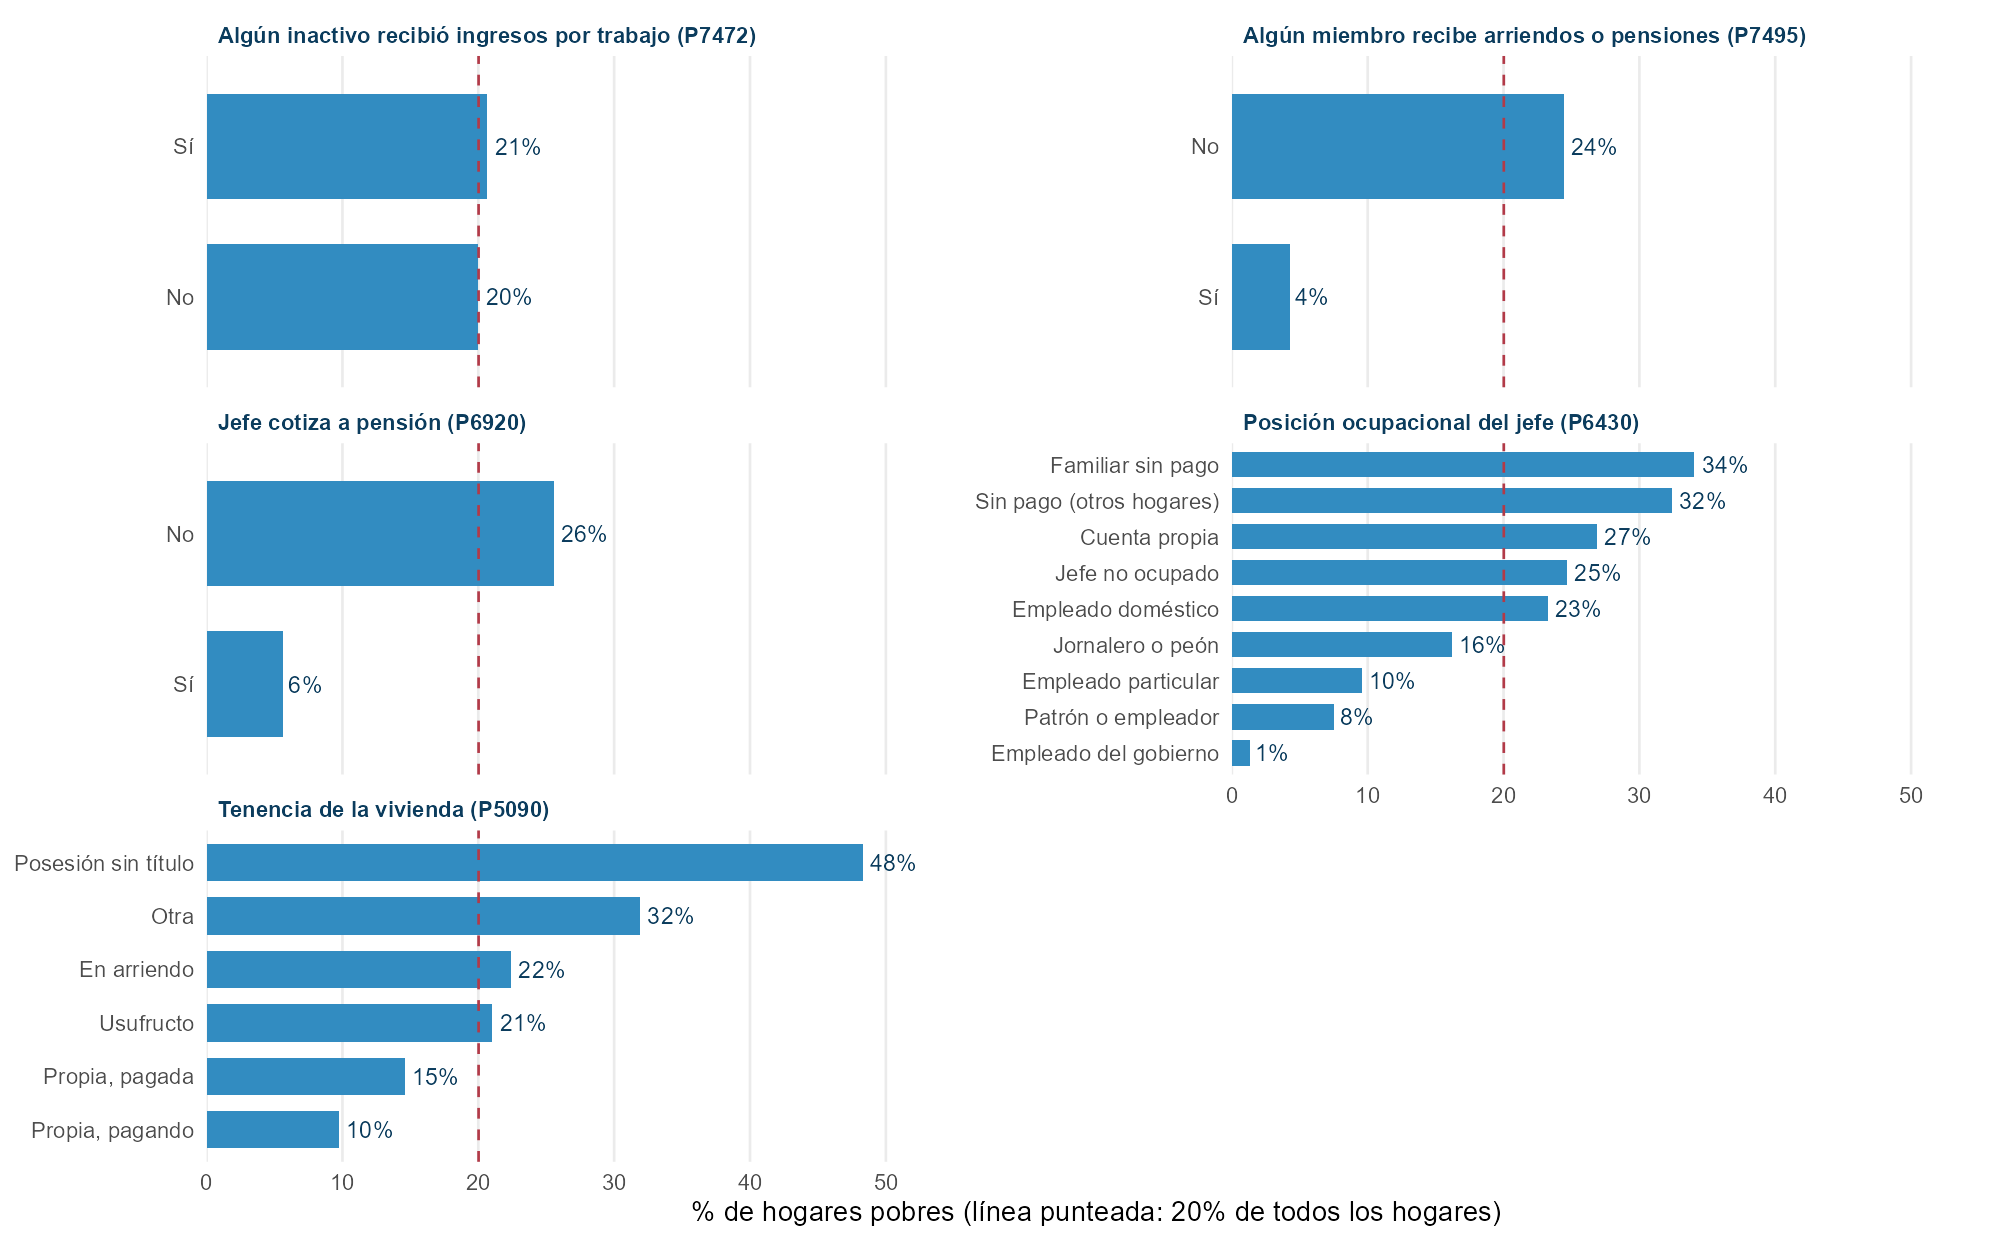
\includegraphics[width=\linewidth, height=0.72\textheight, keepaspectratio]{pres_predictores_cat.png}

\raggedright\footnotesize
Las preguntas con mayor importancia en el modelo
(ver la sección de importancia): la \textbf{posición ocupacional} separa más que
cualquier otra; recibir \textbf{arriendos o pensiones} y la
\textbf{formalidad del jefe} marcan a los hogares no pobres.
\end{frame}

\begin{frame}{Datos: los predictores que importan, continuos}
\begin{columns}[T]
\column{0.64\textwidth}
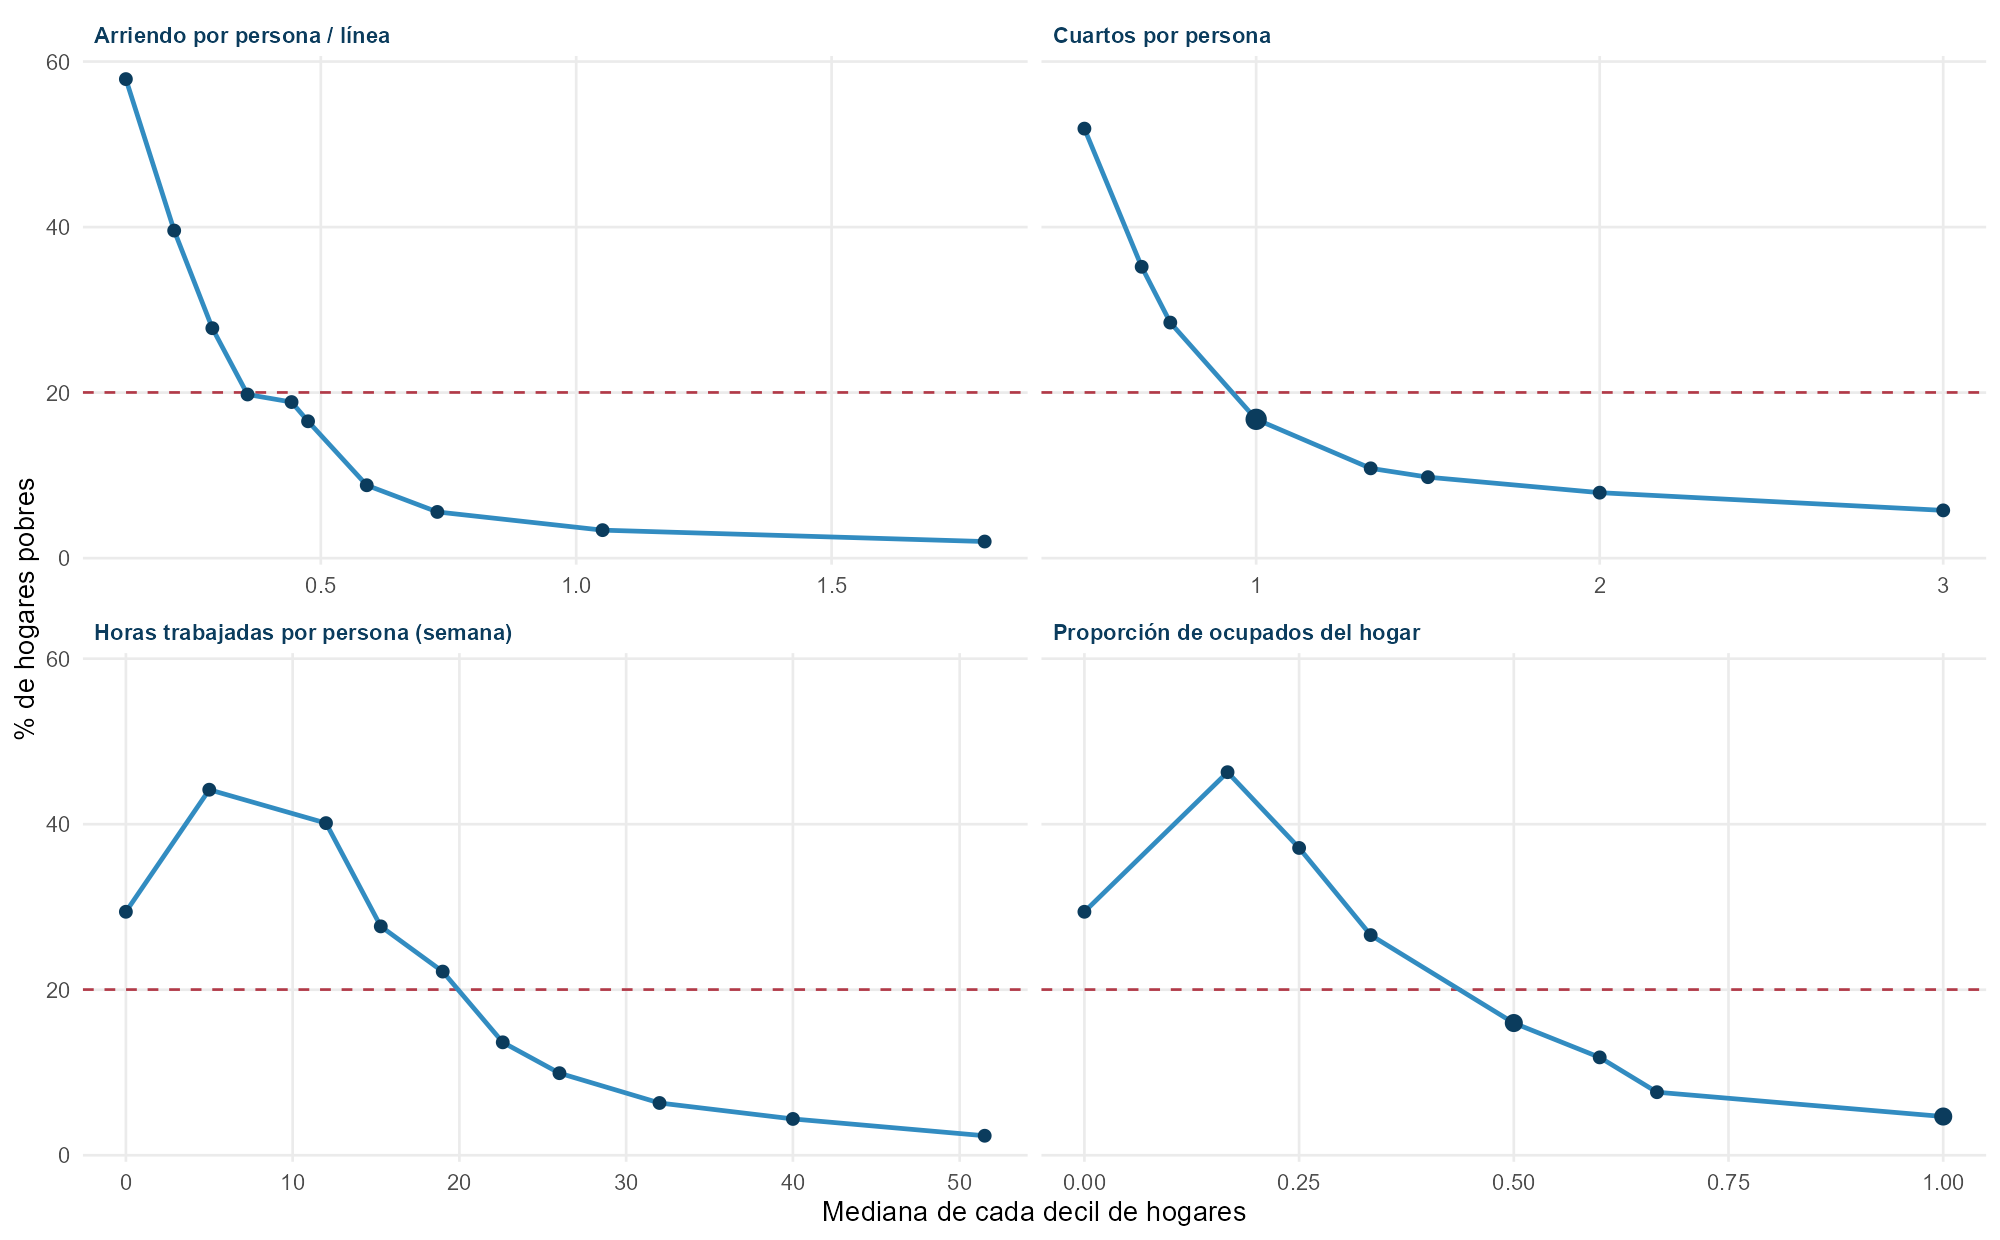
\includegraphics[width=\linewidth]{pres_predictores_cont.png}
\column{0.34\textwidth}
\small
\begin{itemize}
  \item La pobreza cae rápido con el \textbf{arriendo por persona}, las
    \textbf{horas} y los \textbf{ocupados}, y después se aplana:
    relaciones \emph{no lineales} y con umbrales.
  \item Muchos hogares con cero horas u ocupados: una masa en cero que
    un modelo lineal no captura bien.
  \item Esa forma es la que aprovechan los árboles.
\end{itemize}
\footnotesize Línea punteada: 20\% de hogares pobres.
\end{columns}
\end{frame}

\begin{frame}{El pivote: de la persona al hogar}
\begin{columns}[T]
\column{0.56\textwidth}
\begin{tikzpicture}
\begin{axis}[barras, xbar, width=2.9cm, height=5.2cm,
  xmin=0.69, xmax=0.805,
  symbolic y coords={P8,P7,P6,P5,P4,P3,P2,P1}, ytick=data,
  yticklabels={{+ regresión del ingreso (70/30)}, {+ ingreso con Tweedie},
               {+ ingreso afinado y arriendo imputado}, {+ ingresos sin estar ocupado},
               {+ categóricas nativas}, {+ ingreso predicho y stacking},
               {Por hogar: agregados de los miembros}, {Por persona, promediado}},
  xtick={0.70,0.74,0.78},
  xticklabel style={/pgf/number format/fixed, /pgf/number format/precision=2},
  xlabel={\scriptsize $F_1$ de validación cruzada},
  every node near coord/.append style={/pgf/number format/fixed,
    /pgf/number format/precision=4},
  bar width=6pt, enlarge y limits=0.08]
\addplot[fill=azulclaro, draw=azul] coordinates {
  (0.7775,P8) (0.7772,P7) (0.7741,P6) (0.7714,P5)
  (0.7612,P4) (0.7598,P3) (0.7534,P2) (0.7055,P1)};
\end{axis}
\end{tikzpicture}

\column{0.42\textwidth}
\small
\textbf{Fase 1:} modelar a cada persona y promediar en el hogar. Techo de
0,706.

\vspace{2mm}
\textbf{Fase 2 (pivote):} una fila por hogar, con sumas, proporciones y los
datos del jefe: $+0{,}05$ de $F_1$.

\vspace{2mm}
\textbf{Después:} cada escalón agrega \emph{información} sobre el ingreso
del hogar, no combinaciones de variables. Logaritmos, cuadrados, índices e
interacciones no sumaron: los árboles ya las construyen.
\end{columns}
\end{frame}

% =============================================================================
\section{Mejor modelo}
% =============================================================================

\begin{frame}{Estructura del modelo final}
% -----------------------------------------------------------------------------
% PLACEHOLDER: explicación visual de la estructura del modelo.
% Por defecto se incluye el diagrama de latex/estructura_modelo_slide.tex
% (output/figures/estructura_modelo_slide.png).
% -----------------------------------------------------------------------------
\centering
\IfFileExists{../output/figures/estructura_modelo_slide.png}{%
  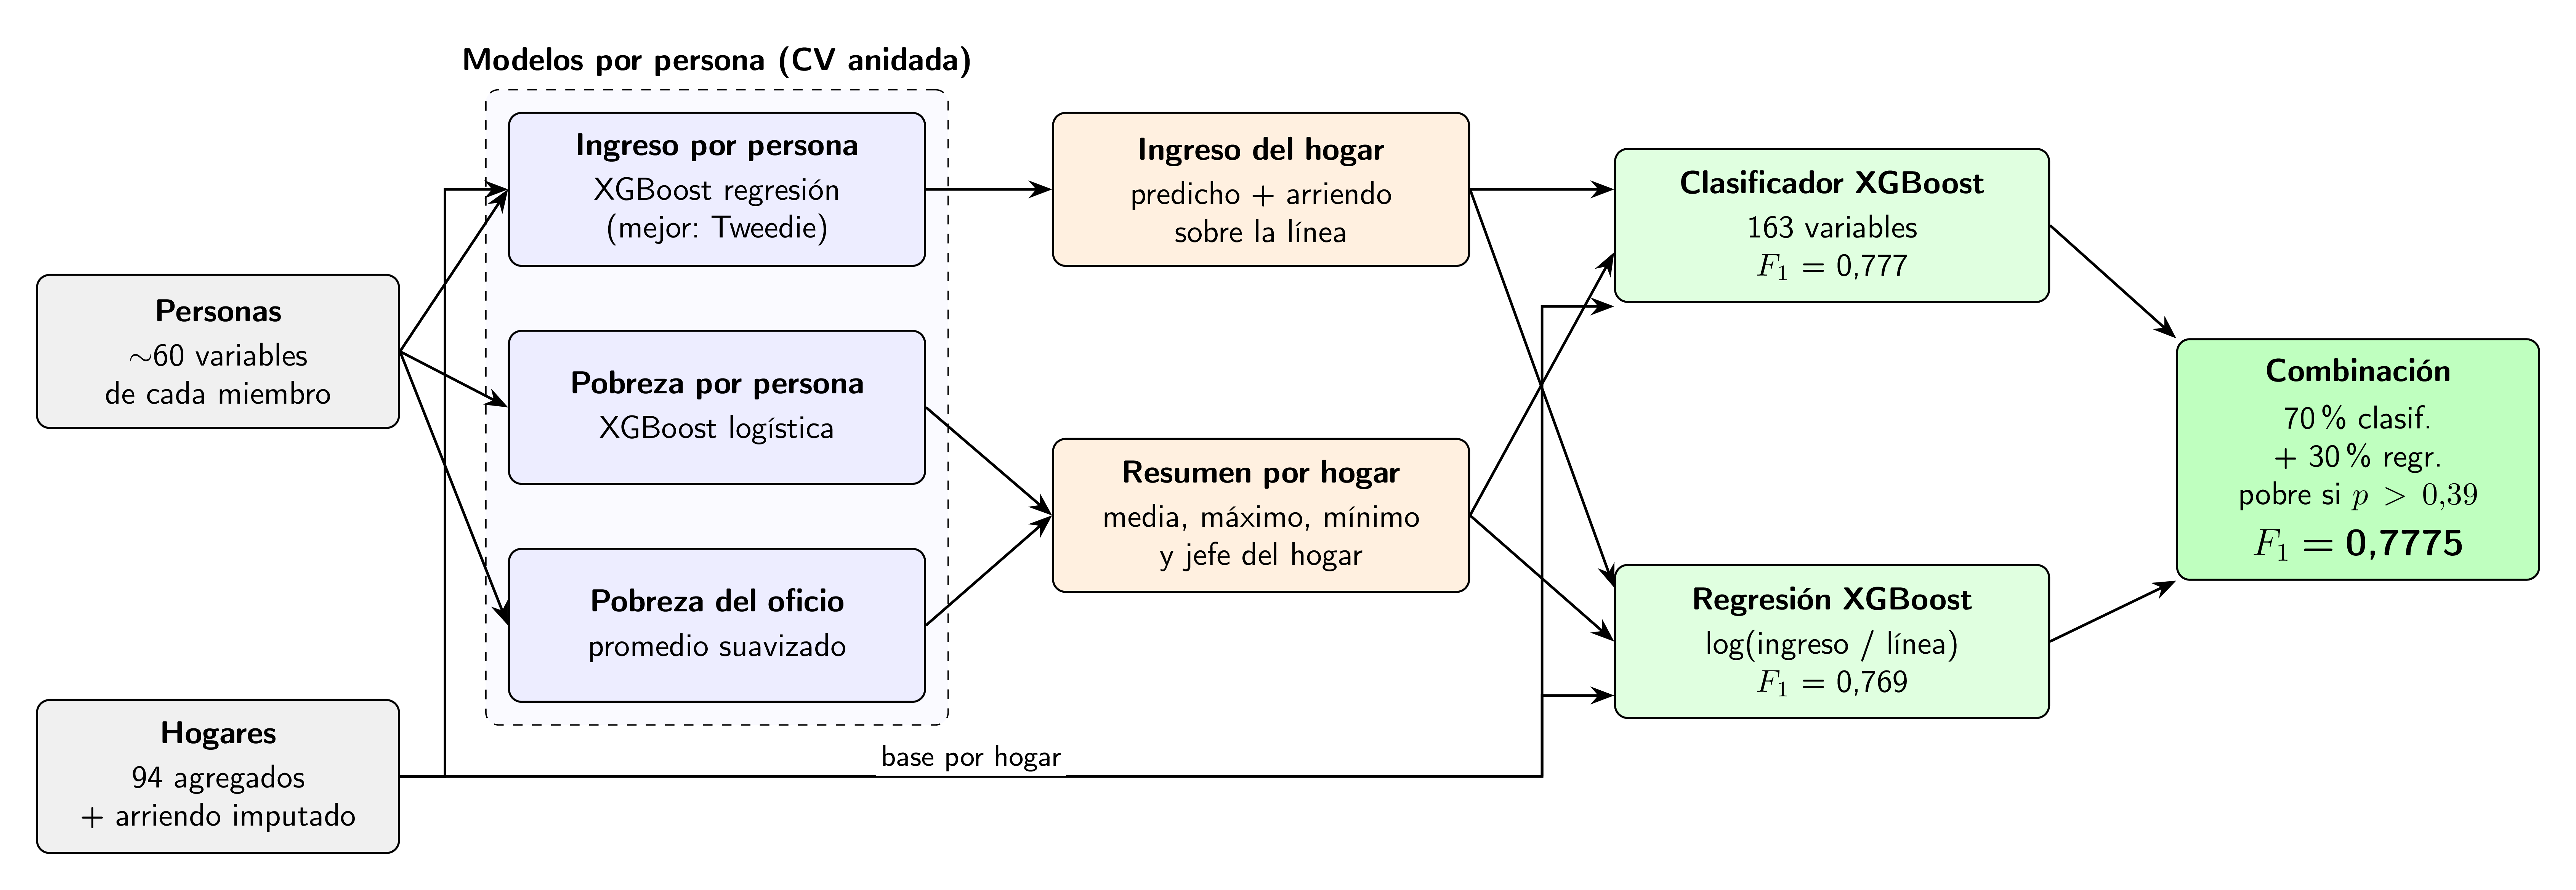
\includegraphics[width=\linewidth, height=0.7\textheight, keepaspectratio]{estructura_modelo_slide.png}%
}{%
  \fbox{\parbox[c][0.6\textheight][c]{0.9\linewidth}{\centering
    \Large [PLACEHOLDER: DIAGRAMA DE LA ESTRUCTURA DEL MODELO]\\[2mm]
    \normalsize Personas $\rightarrow$ modelos auxiliares $\rightarrow$
    resúmenes por hogar $\rightarrow$ clasificador + regresión
    $\rightarrow$ combinación 70/30}}%
}

\vspace{1mm}
\raggedright\footnotesize Tres niveles: (1) modelos por persona con validación
cruzada anidada; (2) resúmenes por hogar (suma, máximo, mínimo, el del jefe);
(3) clasificador y regresión por hogar, combinados.
\end{frame}

\begin{frame}{Parada temprana y umbral}
\begin{columns}[T]
\column{0.48\textwidth}
\tema{Parada temprana: cuántos árboles}\\[1mm]
\begin{tikzpicture}
\begin{axis}[scale only axis, width=4.6cm, height=2.6cm,
  xmin=0, xmax=1200, ymin=0.1, ymax=0.62,
  xlabel={\scriptsize Número de árboles}, ylabel={\scriptsize Log-loss},
  xtick={0,400,800,1200}, ytick=\empty,
  xticklabel style={font=\scriptsize}, axis lines=left]
\addplot[azulclaro, thick, domain=0:1200, samples=60] {0.18 + 0.42*exp(-x/180)};
\addplot[rojo, thick, domain=0:1200, samples=60] {0.235 + 0.37*exp(-x/170) + 0.00000004*max(x-700,0)^2};
\fill[gris!15] (axis cs:740,0.1) rectangle (axis cs:840,0.6);
\draw[dashed, gris] (axis cs:740,0.1) -- (axis cs:740,0.6);
\node[font=\tiny, gris, anchor=north, align=center] at (axis cs:790,0.58) {100\\ más};
\node[font=\tiny, rojo, anchor=south] at (axis cs:1020,0.27) {validación};
\node[font=\tiny, azulclaro, anchor=north] at (axis cs:1020,0.17) {entrenamiento};
\node[font=\tiny, gris, anchor=south] at (axis cs:740,0.6) {mejor árbol};
\end{axis}
\end{tikzpicture}

\footnotesize Cada árbol nuevo corrige el error de los anteriores. Se para
cuando la log-loss del fold de validación lleva \textbf{100 árboles} sin
mejorar, y se usa el mejor (613--869 árboles según el fold). Más árboles
solo memorizan el entrenamiento.

\column{0.5\textwidth}
\tema{Umbral: cuándo decir ``pobre''}\\[1mm]
\begin{tikzpicture}
\begin{axis}[scale only axis, width=4.9cm, height=2.6cm,
  xmin=0.05, xmax=0.95, ymin=0.4, ymax=1,
  xlabel={\scriptsize Umbral}, xtick={0.1,0.39,0.5,0.7,0.9},
  ytick={0.4,0.6,0.8,1},
  xticklabel style={font=\scriptsize, /pgf/number format/fixed},
  yticklabel style={font=\scriptsize, /pgf/number format/fixed},
  axis lines=left, grid=major, grid style={gris!15}]
\addplot[azul, very thick] table[x=umbral, y=f1] {\dat{umbral_final}};
\addplot[verde, thick, dashed] table[x=umbral, y=precision] {\dat{umbral_final}};
\addplot[dorado!85!black, thick, dotted] table[x=umbral, y=recall] {\dat{umbral_final}};
\draw[gris] (axis cs:0.39,0.4) -- (axis cs:0.39,1);
\node[font=\tiny, azul, anchor=south west] at (axis cs:0.40,0.79) {$F_1$};
\node[font=\tiny, verde, anchor=south east] at (axis cs:0.60,0.88) {precisión};
\node[font=\tiny, dorado!85!black, anchor=north east] at (axis cs:0.60,0.62) {recall};
\end{axis}
\end{tikzpicture}

\footnotesize Un hogar se clasifica como pobre si su probabilidad predicha
supera el umbral. Un umbral más alto aumenta la precisión y reduce el
recall. Usamos el umbral con mayor $F_1$ promedio en los 5 folds,
\textbf{0,39}; con 0,5 el $F_1$ sería 0,765.
\end{columns}
\end{frame}

\begin{frame}{Hiperparámetros: qué controla cada uno}
\begin{columns}[T]
\column{0.56\textwidth}
\scriptsize
\setlength{\tabcolsep}{3pt}
\renewcommand{\arraystretch}{1.2}
\begin{tabular}{@{}l>{\centering\arraybackslash}p{0.9cm}>{\raggedright\arraybackslash}p{4.7cm}@{}}
\toprule
Parámetro & Valor & Intuición \\
\midrule
\texttt{eta} & 0,02 & Tamaño del paso: cada árbol corrige solo el 2\% del error. Pasos cortos, más árboles, menos sobreajuste \\
\texttt{max\_depth} & 8 & Hasta 8 preguntas por rama: interacciones de hasta 8 variables (ingreso $\times$ tenencia $\times$ tamaño\ldots) \\
\texttt{min\_child\_weight} & 50 & Una hoja necesita suficiente evidencia ($\approx$ 50 hogares con duda): no se crean reglas para casos aislados \\
\texttt{colsample\_bytree} & 0,5 & Cada árbol ve la mitad de las variables: obliga a usar señales distintas \\
\texttt{subsample} & 0,8 & Cada árbol ve el 80\% de los hogares: más azar, menos varianza \\
árboles & 613--869 & Los fija la parada temprana \\
\texttt{gamma}, \texttt{lambda}, \texttt{alpha} & 0, 1, 0 & Penalizaciones fijas desde iteraciones previas \\
\bottomrule
\end{tabular}

\column{0.42\textwidth}
\centering
\begin{tikzpicture}[font=\tiny,
  nodo/.style={circle, fill=azulclaro, inner sep=1.6pt},
  hoja/.style={rectangle, fill=azul!15, draw=azul, inner sep=1.5pt, minimum width=5mm},
  level distance=6mm, level 1/.style={sibling distance=18mm},
  level 2/.style={sibling distance=9mm}, edge from parent/.style={draw, gris}]
\node[nodo, label=above:{¿ingreso pred.\ $<$ línea?}] {}
  child {node[nodo] {} child {node[hoja] {$\geq$50}} child {node[hoja] {$\geq$50}}}
  child {node[nodo] {} child {node[hoja] {$\geq$50}} child {node[hoja] {$\geq$50}}};
\draw[gris, decorate, |-|] (2.1,-0.05) -- node[right, align=left] {profundidad\\ $\leq$ 8} (2.1,-1.3);
\end{tikzpicture}

\vspace{3mm}
\begin{tikzpicture}[font=\scriptsize,
  arb/.style={rectangle, rounded corners=1pt, draw=azul, fill=azul!8, minimum width=7mm, minimum height=5mm}]
\node[arb] (a1) {$f_1$};
\node[right=1mm of a1] (p1) {$+\,0{,}02\,\times$};
\node[arb, right=1mm of p1] (a2) {$f_2$};
\node[right=1mm of a2] (p2) {$+\cdots+\,0{,}02\,\times$};
\node[arb, right=1mm of p2] (a3) {$f_{M}$};
\node[below=2mm of p1, xshift=8mm, gris, align=center] {cada árbol aprende el error que dejaron los anteriores\\ (columnas y hogares al azar)};
\end{tikzpicture}

\vspace{2mm}
\raggedright\footnotesize La superficie es plana: entre las mejores
combinaciones el $F_1$ solo va de 0,772 a 0,773. Los hiperparámetros
\emph{no} fueron la fuente de la ganancia.
\end{columns}
\end{frame}

\begin{frame}{Funciones de pérdida y pesos de la combinación}
\begin{columns}[T]
\column{0.5\textwidth}
\small
\tema{1. Ingreso por persona con pérdida Tweedie} ($\rho = 1{,}2$; laboral y
no laboral por separado)
\par\vspace{1mm}
{\centering $L(y,\mu) = -\dfrac{y\,\mu^{1-\rho}}{1-\rho} + \dfrac{\mu^{2-\rho}}{2-\rho}$\par}
\vspace{1mm}
\footnotesize Entre la Poisson y la Gamma: admite ceros y una cola larga, y
predice la \emph{media} en pesos. Al sumar a los miembros, el ingreso del
hogar ya no queda subestimado: $R^2$ 0,63 $\to$ 0,66; $F_1$ 0,7733
$\to$ 0,7772.

\vspace{2mm}
\small
\tema{3. Combinación 70/30}
\par\vspace{1mm}
\footnotesize La regresión se pasa a probabilidad con un logit de
\texttt{pobre} sobre su predicción. Luego
$p = w\,p_{\text{clasif.}} + (1-w)\,p_{\text{regr.}}$, con $w$ y el umbral
escogidos juntos por $F_1$: $w = 0{,}7$, umbral 0,39.

\column{0.48\textwidth}
\small
\tema{2. Regresión de $z = \log(\text{ingreso}/\text{línea})$ con pesos}
\par\vspace{1mm}
{\centering $w_i = 1 + 3\,e^{-|z_i|/0{,}25}$\par}
\vspace{1mm}
\centering
\begin{tikzpicture}
\begin{axis}[scale only axis, width=4.6cm, height=2.3cm,
  xmin=-1.5, xmax=1.5, ymin=0.8, ymax=4.3,
  xlabel={\scriptsize $z$ (0 = en la línea)}, ylabel={\scriptsize peso},
  xtick={-1,0,1}, ytick={1,2,3,4},
  ticklabel style={font=\scriptsize}, axis lines=left]
\addplot[azul, very thick, domain=-1.5:1.5, samples=121] {1 + 3*exp(-abs(x)/0.25)};
\draw[dashed, gris] (axis cs:0,0.8) -- (axis cs:0,4.3);
\node[font=\tiny, gris, anchor=east] at (axis cs:-0.1,3.8) {pobre};
\node[font=\tiny, gris, anchor=west] at (axis cs:0.1,3.8) {no pobre};
\end{axis}
\end{tikzpicture}

\raggedright\footnotesize Un hogar en la línea pesa 4; uno al doble de la
línea, casi 1. La regresión se concentra donde se decide la clasificación.
Se escogió entre amplitudes $\{1, 3\}$ y anchos $\{0{,}25;\ 0{,}5\}$.
\end{columns}
\end{frame}

\begin{frame}{Importancia por permutación: qué le resta al modelo quitar cada grupo}
\begin{columns}[T]
\column{0.6\textwidth}
\begin{tikzpicture}
\begin{axis}[scale only axis, width=5.0cm, height=4.6cm,
  xmin=0.3, xmax=0.8, ymin=0.4, ymax=7.6,
  ytick={1,...,7}, yticklabel style={font=\scriptsize, align=right},
  yticklabels={{Tasa de pobreza del oficio}, {Ubicación}, {Otras construidas},
               {Base por hogar (89 agregados)}, {Prob.\ de ser pobre por persona},
               {Prob.\ ingreso $<$ 0,8 / 1,25 líneas}, {Ingreso predicho por persona}},
  xtick={0.35,0.5,0.6,0.7,0.7775}, xticklabels={{0,35},{0,5},{0,6},{0,7},{0,78}},
  xticklabel style={font=\scriptsize},
  xlabel={\scriptsize $F_1$ después de permutar el grupo (línea: 0,7775)},
  axis lines=left, grid=major, grid style={gris!15}]
\draw[dashed, azul] (axis cs:0.7775,0.4) -- (axis cs:0.7775,7.6);
\addplot[only marks, mark=*, mark size=1.8pt, rojo] coordinates {
  (0.7770,1) (0.7753,2) (0.7724,3) (0.7678,4) (0.7338,5) (0.7168,6) (0.3543,7)};
\draw[rojo, thick] (axis cs:0.7775,4) -- (axis cs:0.7678,4);
\draw[rojo, thick] (axis cs:0.7775,5) -- (axis cs:0.7338,5);
\draw[rojo, thick] (axis cs:0.7775,6) -- (axis cs:0.7168,6);
\draw[rojo, thick] (axis cs:0.7775,7) -- (axis cs:0.3543,7);
\begin{scope}[font=\tiny, rojo]
\node[anchor=east] at (axis cs:0.7740,1) {$-$0,0005};
\node[anchor=east] at (axis cs:0.7720,2) {$-$0,002};
\node[anchor=east] at (axis cs:0.7690,3) {$-$0,005};
\node[anchor=east] at (axis cs:0.7640,4) {$-$0,010};
\node[anchor=east] at (axis cs:0.7300,5) {$-$0,044};
\node[anchor=east] at (axis cs:0.7130,6) {$-$0,061};
\node[anchor=north] at (axis cs:0.5600,6.95) {$-$0,423};
\end{scope}
\end{axis}
\end{tikzpicture}

\column{0.38\textwidth}
\small
\begin{itemize}
  \item Se desordena el grupo entre los hogares del fold de validación y se
    mide cuánto cae el $F_1$ (5 folds $\times$ 3 permutaciones).
  \item Sin el \textbf{ingreso predicho}, el $F_1$ cae a 0,35: es el
    corazón del modelo.
  \item La variable individual más importante es la fórmula del DANE con el
    ingreso predicho ($-$0,043).
  \item De 163 variables, \textbf{21 no aportan} o restan: quitarlas no
    cambiaría nada.
\end{itemize}
\end{columns}
\end{frame}

\begin{frame}{Importancia de extremo a extremo: por dónde entra cada concepto}
\begin{columns}[T]
\column{0.62\textwidth}
\begin{tikzpicture}
\begin{axis}[scale only axis, xbar, width=4.6cm, height=4.7cm,
  xmin=-0.06, xmax=0.25, ymin=0.4, ymax=10.6, bar width=7pt, bar shift=0pt, clip=false,
  xticklabel style={font=\scriptsize},
  xtick={-0.05,0,0.05,0.10,0.15,0.20}, xticklabels={{0,05},{0},{0,05},{0,10},{0,15},{0,20}},
  xlabel={\scriptsize Caída del $F_1$},
  axis lines=left, axis y line=none]
\addplot[fill=azul, draw=azul] coordinates {
  (0.010,1) (0.008,2) (0.024,3) (0.017,4) (0.023,5) (0.070,6)
  (0.122,7) (0.045,8) (0.137,9) (0.226,10)};
\addplot[fill=dorado, draw=dorado] coordinates {
  (-0.001,1) (-0.005,2) (-0.006,3) (-0.009,4) (-0.035,5) (0.000,6)
  (-0.005,7) (-0.037,8) (-0.001,9) (-0.002,10)};
\draw[gris] (axis cs:0,0.4) -- (axis cs:0,10.6);
\begin{scope}[font=\scriptsize]
\node[anchor=east] at (axis cs:-0.042,1) {Salud};
\node[anchor=east] at (axis cs:-0.042,2) {Primas, subsidios, especie};
\node[anchor=east] at (axis cs:-0.042,3) {Educación};
\node[anchor=east] at (axis cs:-0.042,4) {Ubicación y línea};
\node[anchor=east] at (axis cs:-0.042,5) {Edad, sexo, tamaño};
\node[anchor=east] at (axis cs:-0.042,6) {Búsqueda de trabajo};
\node[anchor=east] at (axis cs:-0.042,7) {Ocupación y horas};
\node[anchor=east] at (axis cs:-0.042,8) {Vivienda y arriendo};
\node[anchor=east] at (axis cs:-0.042,9) {Ingresos no laborales};
\node[anchor=east] at (axis cs:-0.042,10) {Formalidad, posición, oficio};
\end{scope}
\node[font=\tiny, dorado!85!black, anchor=south] at (axis cs:-0.03,10.6) {directa};
\node[font=\tiny, azul, anchor=south] at (axis cs:0.11,10.6) {vía modelos por persona};
\end{axis}
\end{tikzpicture}

\column{0.36\textwidth}
\small
\begin{itemize}
  \item Se permuta el concepto en las personas y en el hogar, y se recalcula
    toda la cadena.
  \item El \textbf{trabajo} pesa más, y casi todo entra \emph{a través del
    ingreso predicho}.
  \item Solo la \textbf{vivienda} y el \textbf{tamaño} entran directo: la
    fórmula suma el arriendo y divide entre personas.
  \item Educación y salud: $\leq$ 0,024. Su información ya está en el
    trabajo.
\end{itemize}
\footnotesize Los efectos no se suman: los conceptos están correlacionados.
\end{columns}
\end{frame}

\begin{frame}{Por qué importan estos conceptos: la teoría detrás}
\scriptsize
\setlength{\tabcolsep}{5pt}
\renewcommand{\arraystretch}{1.25}
\begin{tabular}{@{}>{\raggedright\arraybackslash}p{2.9cm}>{\raggedright\arraybackslash}p{5.4cm}>{\raggedright\arraybackslash}p{5.3cm}@{}}
\toprule
\textbf{Concepto (caída del $F_1$)} & \textbf{Teoría} & \textbf{Qué implica para el modelo} \\
\midrule
Formalidad, posición y oficio ($-$0,226) &
  \textbf{Lewis (1954)}: en la economía dual, el sector de subsistencia
  absorbe un exceso de trabajadores en tareas de baja productividad, con
  ingresos de subsistencia. &
  La posición ocupacional ubica al hogar en uno de los dos sectores. Sin
  ella el modelo pierde la señal que más separa a pobres de no pobres. \\
Educación ($-$0,021) &
  \textbf{Becker (1964)}: el capital humano aumenta la productividad y abre
  empleos especializados, de mayor valor agregado y más formales. &
  La educación determina el ingreso de largo plazo \emph{a través} del
  empleo: su información ya está en la posición y la formalidad, por eso
  pesa poco sola. \\
Ingresos no laborales ($-$0,143) &
  \textbf{Deaton (1997)}: los hogares vulnerables no viven de un salario
  estable; suavizan su consumo con remesas, transferencias, pensiones y
  ayudas. &
  Por eso estas preguntas entran a los modelos por persona: identifican
  quién tiene ingresos sin estar ocupado. \\
Ingresos irregulares (errores cerca de la línea) &
  \textbf{Collins et al.\ (2009)}: los hogares pobres manejan flujos
  irregulares con crédito informal, ahorro y deudas que pagan
  constantemente. &
  Un mes de encuesta no refleja su ingreso permanente: cerca de la línea,
  el error es en buena parte irreducible. \\
\bottomrule
\end{tabular}
\vspace{1mm}

\footnotesize
\textbf{Quién se detecta mejor:} los pobres informales, con poca
educación y en hogares grandes encajan en el sector de subsistencia de
Lewis. Los pobres con jefe formal o educado ``no lo parecen'' según Becker,
y el modelo los excluye más (recall de 65\%).
\end{frame}

\begin{frame}{Qué sumó y qué restó en el camino}
\begin{columns}[T]
\column{0.64\textwidth}
\begin{tikzpicture}
\begin{axis}[scale only axis, xbar, width=4.0cm, height=5.4cm,
  xmin=-0.0115, xmax=0.0125, ymin=0.3, ymax=13.7, bar width=5pt, bar shift=0pt,
  ytick={1,...,13},
  yticklabels={{Base aumentada (pobres replicados)}, {Logaritmos y cuadrados},
               {Regresión como variable}, {Índices de variables débiles},
               {Modelo especialista cerca de la línea}, {Más peso cerca de la línea},
               {Regresión del ingreso (70/30)}, {Arriendo imputado (regla DANE)},
               {Categóricas nativas}, {Ingreso afinado con preguntas nuevas},
               {Pérdida Tweedie}, {Ingreso predicho y stacking},
               {Ingresos sin estar ocupado}},
  yticklabel style={font=\scriptsize}, xticklabel style={font=\scriptsize},
  scaled x ticks=false, xtick={-0.006,0,0.006},
  xticklabels={{$-$0,006},{0},{+0,006}}, xlabel={\scriptsize Cambio en el $F_1$},
  axis x line=bottom, axis y line=left, y axis line style={draw=none},
  nodes near coords, point meta=x, every node near coord/.append style={font=\tiny,
    /pgf/number format/fixed, /pgf/number format/precision=4, /pgf/number format/showpos}]
\addplot[fill=rojo, draw=rojo] coordinates {
  (-0.0062,1) (-0.0010,2) (-0.0008,3) (-0.0007,4) (-0.0007,5) (-0.0003,6)};
\addplot[fill=verde, draw=verde] coordinates {
  (0.0003,7) (0.0008,8) (0.0014,9) (0.0016,10) (0.0031,11) (0.0061,12) (0.0092,13)};
\draw[gris] (axis cs:0,0.3) -- (axis cs:0,13.7);
\end{axis}
\end{tikzpicture}

\column{0.34\textwidth}
\small
\begin{itemize}
  \item \textcolor{verde}{\textbf{Sumó}}: todo lo que mejora la
    \emph{medición del ingreso} del hogar.
  \item \textcolor{rojo}{\textbf{Restó o no cambió}}: más
    transformaciones de las mismas variables, rebalancear la muestra y
    modelos extra cerca de la línea.
  \item Cambios de menos de 0,001 están dentro del ruido entre
    particiones.
\end{itemize}
\footnotesize Cada barra compara con el mejor modelo de ese momento
(cuadros de \texttt{resultados.tex}).
\end{columns}
\end{frame}

\begin{frame}{Diagnósticos: dónde se equivoca el modelo}
\begin{columns}[T]
\column{0.6\textwidth}
\begin{tikzpicture}
\begin{axis}[scale only axis, ybar stacked, width=5.6cm, height=3.6cm,
  ymin=0, ymax=50, bar width=9pt, xtick=data,
  xticklabels from table={\dat{errores_linea}}{grupo},
  xticklabel style={font=\tiny, rotate=45, anchor=north east},
  yticklabel style={font=\scriptsize}, ylabel={\scriptsize \% de los hogares del grupo},
  xlabel={\scriptsize Ingreso / línea},
  axis lines=left, grid=major, grid style={gris!15}]
\addplot[fill=rojo, draw=rojo] table[x=posicion, y expr=100*\thisrow{fn}/\thisrow{hogares}] {\dat{errores_linea}};
\addplot[fill=dorado, draw=dorado] table[x=posicion, y expr=100*\thisrow{fp}/\thisrow{hogares}] {\dat{errores_linea}};
\draw[dashed, gris] (axis cs:5.5,0) -- (axis cs:5.5,50);
\node[font=\tiny, rojo, anchor=south east] at (axis cs:5.3,46) {pobres excluidos};
\node[font=\tiny, dorado!85!black, anchor=south west] at (axis cs:5.7,46) {no pobres incluidos};
\end{axis}
\end{tikzpicture}

\column{0.38\textwidth}
\small
\begin{itemize}
  \item A cada lado de la línea el modelo falla en \textbf{cerca de 4 de
    cada 10} hogares; al doble de la línea, casi nunca.
  \item Los errores se reparten: a la izquierda excluye pobres, a la
    derecha incluye no pobres.
  \item Ni más peso cerca de la línea ni un modelo especialista lo
    corrigen: con estas preguntas, ese error es \textbf{irreducible}.
\end{itemize}
\end{columns}
\end{frame}

% =============================================================================
\section{Implicaciones de política}
% =============================================================================

\begin{frame}{Del $F_1$ a la focalización: leakage vs.\ undercoverage}
\begin{columns}[T]
\column{0.42\textwidth}
\small
Umbral 0,39, predicciones fuera de muestra:
\begin{itemize}
  \item \textbf{Cobertura} $\approx$81\% $\Rightarrow$
    \textbf{undercoverage} $\approx$19\%.
  \item \textbf{Precisión} $\approx$75\% $\Rightarrow$ \textbf{leakage}: 1 de
    cada 4 beneficiarios no es pobre.
  \item El $F_1$ pesa igual los dos errores; un programa no tiene por qué:
    el umbral es una \textbf{decisión de política}.
\end{itemize}
\footnotesize
Rural, informal y hogares grandes: más \emph{inclusión}. Pobres ``que no lo
parecen'' (jefe formal o educado, hogar pequeño): más \emph{exclusión}. Jefa
mujer: +3,8 pp de detección. Son tasas base distintas, no una regla
discriminatoria (Kleinberg et al., 2017).

\column{0.55\textwidth}
\scriptsize
\setlength{\tabcolsep}{4pt}
\begin{tabular}{@{}llrrr@{}}
\toprule
Atributo & Grupo & \% pobres & Sensib. & Falsos pos. \\
\midrule
Sexo del jefe & Hombre & 18,3 & 78,9 & 6,2 \\
              & Mujer  & 22,4 & 82,7 & 7,4 \\
\midrule
Empleo del jefe & Formal   &  5,6 & \textbf{65,1} &  1,7 \\
                & Informal & 26,1 & 80,2 & \textbf{10,1} \\
\midrule
Zona & Cabecera & 19,0 & 80,8 &  6,2 \\
     & Rural    & 30,0 & 80,0 & \textbf{12,6} \\
\midrule
Educación jefe & Superior & 7,3 & \textbf{65,4} & 2,3 \\
               & Primaria o menos & 28,8 & 83,4 & 10,8 \\
\midrule
Tamaño & 1 o 2 personas & 10,7 & \textbf{66,5} & 3,8 \\
       & 5 o más        & 35,8 & 88,8 & \textbf{12,1} \\
\bottomrule
\end{tabular}
\end{columns}
\end{frame}

\begin{frame}{Pobreza monetaria, focalización y costo de operación}
\begin{columns}[T]
\column{0.48\textwidth}
\small
\tema{Qué mide el modelo}
\begin{itemize}
  \item Solo \textbf{pobreza monetaria}: educación, salud y subsidios casi
    no aportan una vez se conoce el trabajo.
  \item IPM y pobreza monetaria capturan privaciones distintas (Angulo et
    al., 2016): focalizar ingreso con indicadores de salud o educación
    genera errores.
  \item Proxies observables son manipulables (Camacho y Conover, 2011).
\end{itemize}

\column{0.5\textwidth}
\small
\tema{¿Encuesta corta y barata?}
\begin{itemize}
  \item[\textcolor{verde}{+}] No pregunta \textbf{montos de ingreso} (lo más
    caro y subdeclarado): basta el módulo laboral, la vivienda y fuentes de
    ingreso sí/no.
  \item[\textcolor{rojo}{--}] Necesita el módulo laboral de \emph{cada
    miembro} ($\sim$60 preguntas por persona): costo similar a una visita
    SISBÉN.
  \item[\textcolor{rojo}{--}] Formalidad verificable con PILA; ingresos no
    laborales y búsqueda de trabajo, no.
  \item[\textcolor{gris}{$\bullet$}] Reentrenar si cambian la línea o el
    mercado laboral (datos de 2018).
\end{itemize}
\end{columns}
\end{frame}

\begin{frame}{Cierre: qué nos hizo ganar}
\begin{columns}[T]
\column{0.31\textwidth}
\tema{Validación}\\[1mm]
\small Folds por hogar, validación cruzada anidada sin fuga, la misma
partición para comparar todo y otras particiones para confirmar.
Decidimos con la validación cruzada.
\column{0.31\textwidth}
\tema{Uso de las herramientas}\\[1mm]
\small Categóricas nativas, pérdida Tweedie, stacking con modelos por
persona, parada temprana y pesos cerca de la línea.
\column{0.31\textwidth}
\tema{Intuición económica}\\[1mm]
\small Modelar el hogar, predecir el ingreso y reconstruir la regla del
DANE con el arriendo imputado, y buscar en el cuestionario los ingresos
sin empleo.
\end{columns}
\vspace{8mm}
\begin{center}
\large Con la IA, cualquiera combina variables. \\[1mm]
\textbf{La ventaja está en saber qué predecir y en cómo comprobarlo.}
\end{center}
\end{frame}

% =============================================================================
\begin{frame}{Referencias}
\tiny
\begin{list}{}{\leftmargin=1.6em \itemindent=-1.6em \itemsep=1.5pt \parsep=0pt}
  \item Angulo, R., Díaz, Y. y Pardo, R. (2016). The Colombian
    Multidimensional Poverty Index: Measuring poverty in a public policy
    context. \emph{Social Indicators Research, 127}(1), 1--38.
  \item Becker, G. S. (1964). \emph{Human capital: A theoretical and
    empirical analysis, with special reference to education}. National
    Bureau of Economic Research y Columbia University Press.
  \item Camacho, A. y Conover, E. (2011). Manipulation of social program
    eligibility. \emph{American Economic Journal: Economic Policy, 3}(2),
    41--65.
  \item Chen, T. y Guestrin, C. (2016). XGBoost: A scalable tree boosting
    system. En \emph{Proceedings of the 22nd ACM SIGKDD} (pp.\ 785--794).
  \item Collins, D., Morduch, J., Rutherford, S. y Ruthven, O. (2009).
    \emph{Portfolios of the poor: How the world's poor live on \$2 a day}.
    Princeton University Press.
  \item CONPES 3877 (2016). \emph{Declaración de importancia estratégica del
    Sistema de Identificación de Potenciales Beneficiarios (SISBÉN IV)}. DNP.
  \item DANE (2019). \emph{Pobreza monetaria y multidimensional en Colombia
    2018} [Boletín técnico].
  \item DANE y DNP (2012). \emph{Misión para el Empalme de las Series de
    Empleo, Pobreza y Desigualdad (MESEP): metodología de pobreza monetaria}.
  \item Deaton, A. (1997). \emph{The analysis of household surveys: A
    microeconometric approach to development policy}. Johns Hopkins
    University Press y Banco Mundial.
  \item Fernández, C. y Villar, L. (2017). The impact of lowering the payroll
    tax on informality in Colombia. \emph{Economía, 18}(1), 125--155.
  \item Grosh, M. y Baker, J. (1995). \emph{Proxy means tests for targeting
    social programs} (LSMS Working Paper 118). Banco Mundial.
  \item Kleinberg, J., Ludwig, J., Mullainathan, S. y Obermeyer, Z. (2015).
    Prediction policy problems. \emph{American Economic Review, 105}(5),
    491--495.
  \item Kleinberg, J., Mullainathan, S. y Raghavan, M. (2017). Inherent
    trade-offs in the fair determination of risk scores. En \emph{8th
    Innovations in Theoretical Computer Science Conference (ITCS)}.
  \item Lewis, W. A. (1954). Economic development with unlimited supplies of
    labour. \emph{The Manchester School, 22}(2), 139--191.
  \item Ravallion, M. (2016). \emph{The economics of poverty: History,
    measurement, and policy}. Oxford University Press.
\end{list}
\end{frame}

\end{document}
